\documentclass[runningheads,a4paper,12pt]{report}
\usepackage{graphicx,color,verbatim}
\usepackage{amsmath,amssymb,cite,tabularx,booktabs}
\usepackage{algorithmic, algorithm}
\usepackage{appendix}
\usepackage[pdftex,bookmarks=true]{hyperref}
\usepackage{fancyhdr}
%\usepackage{StyleFiles/watermark}

%====Page Setting==========
\setlength{\topmargin}{-0.4in}
\setlength{\topskip}{-3in}    			% between header and text
\setlength{\textheight}{9.5in} 	  	% height of main text
\setlength{\textwidth}{5.5in}     	% width of text
\setlength{\oddsidemargin}{0.75in} 	% odd page left margin
\setlength{\evensidemargin}{0.75in} % even page left margin
\renewcommand{\baselinestretch}{1.66}
%\pagestyle{myheadings}


\newtheorem{theorem}{Theorem}
\newtheorem{definition}{Definition}
\newtheorem{example}{Example}


\begin{document}

%=========Title Page==============


\begin{titlepage}
	\begin{center}
	\large{\textbf{Comparison of Intrusion Detection Systems for Low-Powered Devices}}
	\end{center}

	\begin{center}
	\small{\textit{A project report submitted} \\ \textit{to} \\\textbf{MANIPAL ACADEMY OF HIGHER EDUCATION} \\}
	\end{center}

%	\begin{figure}[h]
%	\begin{center}

%	\includegraphics[height=2.5cm]{mu}
%	\end{center}
%	\end{figure}	%
	\vspace{-0.5cm}
	\begin{center}
	\small{\textit{For Partial Fulfillment of the Requirement for the\\ Award of the Degree\\of}} \\
	\textbf{Bachelor of Technology} \\ \textit{in} \\ \textbf{Computer and Communication Engineering}
	\end{center}

	\begin{center}
	\small{\textit{by}} \\
	\textbf{Pratyay Amrit} \\ \textbf{Reg. No. 140953430} \\
	\end{center}

	\begin{center}
	\small{\textit{Under the guidance of}} \\
\renewcommand{\baselinestretch}{1}
%{
\begin{table}[h]
	\centering
		\begin{tabular}{ c }
            Ms. Ipsita Upasana \\
    		Assistant Professor \\
    		Department of I \& CT \\
    		 Manipal Institute of Technology \\
    		Manipal, India
		\end{tabular}
\end{table}
%}
	\end{center}
	\begin{figure}[h]
  \begin{center}
	%\includegraphics[height=2.8cm]{MITLogoNew}
	
\includegraphics[scale=1]{MITLogo}
	\end{center}
	\end{figure}
	\begin{center}
	\textbf{MAY 2018}
	\end{center}
\end{titlepage}
%===========End of Title Page===========================

%\pagenumbering{roman}
\setcounter{secnumdepth}{3}
\setcounter{tocdepth}{3}

\pagenumbering{roman}
%===================Dedication=================
\begin{center}
I dedicate my thesis to my friends and family.
\end{center}

%=============================================

\begin{center}
\large{\textbf{DECLARATION}}\\
\vspace{1cm}
\end{center}

I hereby declare that this project work entitled \textbf{Intrusion Detection Systems for Use in Low-Powered Devices} is original and has been carried out by
me in the Department of Information and Communication Technology of Manipal Institute of Technology, Manipal, under the guidance of \textbf{Ms. Ipsita Upasana}, \textbf{Assistant Professor}, Department of Information and Communication Technology, M. I. T., Manipal. No part of this work has been submitted for the award of a degree or diploma either to this University or to any other Universities.

\vspace{2cm}

\begin{flushleft}
Place: Manipal\\
Date : 05-05-18
\end{flushleft}


\begin{flushright}
Pratyay Amrit
\end{flushright}

\begin{figure}[bpht!]
  \begin{center}
	
\includegraphics[scale=1]{MITLogo}
	\end{center}
	\end{figure}
%%======================================
%=============Certificate=================
\begin{center}
\large{\textbf{CERTIFICATE}}\\
\end{center}
%%========================================


This is to certify that this project entitled \textbf{Comparison of Intrusion Detection Systems for Use in Low-Powered Devices} is a bonafide project work done by Mr. Pratyay Amrit at Manipal Institute of Technology, Manipal, independently under my guidance and supervision for the award of the Degree of
Bachelor of Technology in Computer and Communication Engineering.


\vspace{4cm}

\begin{table}[h]
	\centering
		\begin{tabular}{p{3in} p{3in}}
			Ms. Ipsita Upasana &  Dr.Balachandra  \\
			Assistant Professor & Professor \& Head \\
			  Department of I \& CT&  Department of I \& CT \\
			Manipal Institute of Technology  & Manipal Institute of Technology\\
			Manipal, India &  Manipal, India
		\end{tabular}
\end{table}

\addcontentsline{toc}{chapter}{Acknowledgements}
%===================Acknowledgements============
\begin{center}
\large{\textbf{ACKNOWLEDGEMENTS}}\\
\vspace{1cm}
\end{center}
I would like to express my special thanks to Dr. Srikant Rao, Director, MIT as well as the Head of Department of Information \& Communication Technology, Dr. Balachandra for giving me the opportunity to conduct this study.\\
My sincere thanks to Ms. Ipsita Upasana, and all faculty members of the Department of Information \& Communcation Technology for providing necessary guidance and feedback throughout the course of the project.

%===============================================

\addcontentsline{toc}{chapter}{Abstract}
%================Thesis Abstract===============
\begin{center}
\Large{\textbf{ABSTRACT}}\\
\end{center}
%=============================================
Intrusion Detection Systems have become an essential part of computer network security. It acts as a first-line defense from cyber-attacks by analyzing the various attributes of a data packet and identifying it as a malicious, or an ordinary one. Such systems have come a long way and in the present time, promise acceptable performance. However, the algorithms that run at the core of these systems are computationally expensive, making them fairly accurate, but almost unimplementable in very low powered devices, such as nodes of a WSAN, or in an IoT based setup. This work attempts to rank various machine learning and data mining techniques on the basis of their accuracy and time required to train and classify network data.

% Refer to ACM Computing Classification System Taxonomy, read first page and following the instruction given therein.=============
\par
\textbf{[Security and Privacy]}: Intrusion/Anomaly Detection and Malware Mitigation--Intrusion detection systems

\tableofcontents
\listoftables
\addcontentsline{toc}{chapter}{List of Tables}
\listoffigures
\addcontentsline{toc}{chapter}{List of Figures}
\addcontentsline{toc}{chapter}{Abbreviations}
%============Abbreviations=========
\begin{center}
\large{\textbf{ABBREVIATIONS}}\\
\vspace{1cm}
%PAPR: Peak-to-Average Power Ratio
\end{center}

\begin{table}[bpht!]
\centering
	\begin{tabular}{lcl}
	IDS&:& Intrusion Detection System\\
    UNSW-NB15&:& University of New South Wales, Network Based 2015 Dataset\\
    KDD'99&:& Knowledge Discovery and Data Mining Competition 1999 Dataset\\
    SIEM&:& System Information and Event Management\\
    KNN&:& K-Nearest Neighbors\\
    NB&:& Gaussian Naive Bayes \\
    DT&:& Decision Tree \\
    DT\_n&:& Decision Tree with max-depth = n \\
    RF\_n&:& Random Forests with max-depth = n \\
    ET\_n&:& Extra Trees with max-depth = n\\
    TP&:& True Positive\\
    TN&:& True Negative\\
    FP&:& False Positive\\
    FN&:& False Negative\\
    TTF&:& Time to Fit \\
    TTP&:& Time to Predict \\
    TS&:& Training Score\\
    PS&:& Prediction Score
	\end{tabular}
\end{table}

\addcontentsline{toc}{chapter}{Notations}
%===========Notations Used=================
\begin{center}
\Large{\textbf{NOTATIONS}}\\
\end{center}
%===============
\begin{table}[bpht!]
\centering
\begin{tabular}{lcl}
$\alpha$&:&Smoothing factor for words\\
$\beta$&:& Smoothing factor for topics
\end{tabular}
\end{table}

\pagenumbering{arabic}

\chapter{Chapter Title}
\label{ch:INTR}
\section{Section 1}
Electronic reference is given in \cite{sh07}. Journal article is given in \cite{odo95}. Article from conference is given in \cite{gs97}. Material from book \cite{cu72}. Manual detail is given in \cite{mo96}. Detail of technical report is given in \cite{jrc87}. A master thesis \cite{ka99} has been referred. A PhD thesis \cite{li2000} has been referred. Last referenec is taken from \cite{ro94}.
\begin{definition}
vvhffff
\end{definition}

\begin{figure}[bpht]
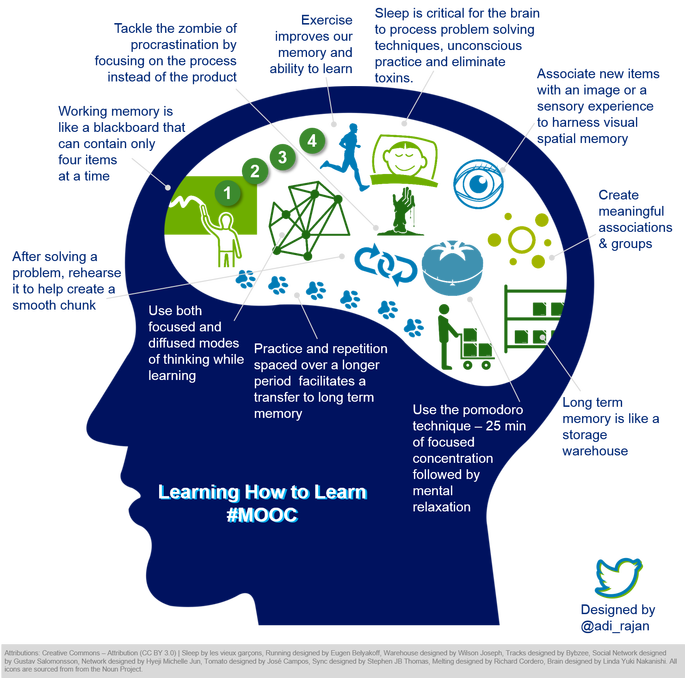
\includegraphics{Chapter1/LHTL}
\caption{Learning how to learn}
\end{figure}

\begin{definition}
fffffff
\end{definition}

\chapter{Literature Review}
\label{ch:LR}
\section{Taxonomy for Intrusion Detection Systems}

\paragraph{}
In \cite{ids_taxonomy}, an attempt has been made to standardize a terminology for IDSs. Many different types of common in-use IDSs are introduced in the paper, along with some upcoming possibilities.

\paragraph{}
Broadly, IDSs have been classified on the basis of 5 different features (Figure \ref{types_of_ids}) \cite{ids_taxonomy}.
\begin{figure}[h]
    \hfill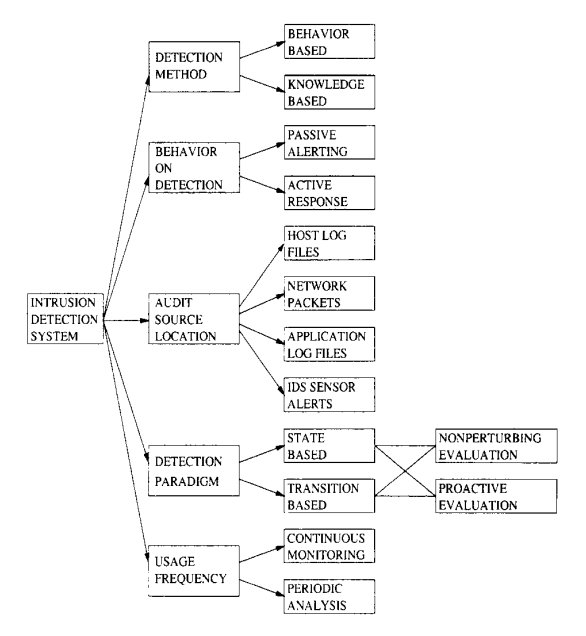
\includegraphics[width=0.8\textwidth]{Chapter2/types_of_ids}\hspace*{\fill}
    \caption{Types of IDS}
    \label{types_of_ids}
\end{figure}
\begin{enumerate}
    \item On the basis of detection method:
        \begin{itemize}
            \item Behavior based
            \item Knowledge based
        \end{itemize}
    \item On the basis of behavior on detection:
        \begin{itemize}
            \item Passive filtering
            \item Active filtering
        \end{itemize}
    \item On the basis of audit source location:
        \begin{itemize}
            \item Host log files
            \item Network packets
            \item Application log files
            \item IDS sensor alerts
        \end{itemize}
    \item On the basis of detection paradigm:
        \begin{itemize}
            \item State based
            \item Transition based
        \end{itemize}
    \item On the basis of usage frequency:
        \begin{itemize}
            \item Continuous monitoring
            \item Periodic analysis
        \end{itemize}
\end{enumerate}

\paragraph{}
This work focuses only on behavior based IDSs. Various methods have been proposed using all kinds of machine learning models, some of which have been tested and compared in this work.

\section{Datasets}

\paragraph{}
When it comes to training and testing IDSs, the KDD'99 \cite{kdd99} and UNSW-NB15 \cite{unsw15} datasets are usually considered.
\begin{itemize}
    \item \textbf{KDD'99}: The KDD'99 dataset was curated in 1999 and was used for The Third International Knowledge Discovery and Data Mining Tools Competition 1999. It holds its popularity till date for training and testing models based on data mining and machine learning algorithms for extracting information out of network packet data. The dataset contained 41 features along with a label mentioning the type of attack detected. The dataset is a raw dump of network traffic, and barely processed for use in machine learning.
    \item \textbf{UNSW-NB15}: The UNSW-NB15 dataset was generated in 2015, and similar to KDD'99, is a dump of network traffic. However, it has been proccessed to fix the problems of KDD'99 \cite{unsw_comparison}. The dataset has a total of 49 features, including 2 class labels and over 2 million records. Since the dataset was generated more recently (2015), it is a more accurate example of network data traffic that an IDS might face in the current times. The class labels have classified 9 different kinds of attacks, some of which were not present in the KDD'99 dataset.
\end{itemize}

\paragraph{}
The UNSW-NB15 proves to be a better dataset for use in this work, owing to its novelty and problems in KDD'99 that it addresses \cite{unsw_comparison}.

\section{UNSW-NB15}
\label{unsw_details}

\paragraph{}
The UNSW-NB15 dataset was released in 2015. It was generated using tcpdump tool to capture about 100GB of raw data. It has the following 9 types of attacks:
\begin{enumerate}
    \item Fuzzers: Fuzzing, or Fuzz Testing is a black box testing technique which aims at finding implementation bugs by injecting malformed or semi-malformed data in an automated fashion. Potential attackers may run fuzz tests on the network to find vulnerabilities that can be exploited.
    \item Analysis: Traffic analysis is a special type of inference attack technique that looks at communication patterns between entities in a system. Knowing who's talking to whom, when, and for how long, can sometimes clue an attacker in to information of which you'd rather she not be aware.
    \item Backdoor: A backdoor is a malware type that negates normal authentication procedures to access a system.\\
    Webserver backdoors are used for a number of malicious activities, including:
    \begin{itemize}
        \item Data theft
        \item Website defacing
        \item Server hijacking
        \item The launching of distributed denial of service (DDoS) attacks
        \item Infecting website visitors (watering hole attacks)
        \item Advanced persistent threat (APT) assaults
    \end{itemize}
    \item DoS: Denial of Service (DoS) is an attack which aims to make a host machine unavailable to its intended users by temporarily or indefinitely disrupting the host machines connection to the internet. \\
    Broadly, DoS attacks can be classified into 3 types:
    \begin{itemize}
        \item Volume Based Attacks: Includes UDP floods, ICMP floods, and other spoofed-packet floods. The attack’s goal is to saturate the bandwidth of the attacked site, and magnitude is measured in bits per second (Bps).
        \item Protocol Attacks: Includes SYN floods, fragmented packet attacks, Ping of Death, Smurf DDoS and more. This type of attack consumes actual server resources, or those of intermediate communication equipment, such as firewalls and load balancers, and is measured in packets per second (Pps).
        \item Application Layer Attacks: Includes low-and-slow attacks, GET/POST floods, attacks that target Apache, Windows or OpenBSD vulnerabilities and more. Comprised of seemingly legitimate and innocent requests, the goal of these attacks is to crash the web server, and the magnitude is measured in Requests per second (Rps).
    \end{itemize}
    \item Exploit: An exploit is a piece of software, a chunk of data, or a sequence of commands that takes advantage of a bug or vulnerability to cause unintended or unanticipated behavior to occur on computer software, hardware, or something electronic.
    \item Generic: This subset contains any general type of attack such as:
    \begin{itemize}
        \item Probe, which is a program or a device inserted into the network to monitor the network and collect data.
        \item User to Root Attacks (U2R), in which an attacker or a hacker tries to get the access rights from a normal host in order, for instance, to gain the root access to the system.
        \item Remote to Local Attacks (R2L), in which a remote user sends data packets to a machine over the internet, which he/she does not have the access to, in order to expose vulnerabilities and exploit privileges which a local user would have on the computer.
    \end{itemize}
    \item Reconnaissance: Active reconnaissance is a type of computer attack in which an intruder engages with the targeted system to gather information about vulnerabilities.
    \item Shellcode: A shellcode is a small piece of code used as the payload in the exploitation of a software vulnerability.
    \item Worm: A computer worm is a standalone malware computer program that replicates itself in order to spread to other computers. Often, it uses a computer network to spread itself, relying on security failures on the target computer to access it.
\end{enumerate}
\paragraph{}
The dataset contains 2,540,044 records with 49 features categorized into 6 categories.
\begin{enumerate}
\item \textbf{Flow Features:} \\
    1. srcip: Source IP address. \\
    2. sport: Source port number. \\
    3. dstip: Destinations IP address. \\
    4. dsport: Destination port number. \\
    5. proto: Protocol type, such as TCP, UDP.
\item \textbf{Basic Features:} \\
    6. state: The states and its dependent protocol e.g., CON. \\
    7. dur: Row total duration. \\
    8. sbytes: Source to destination bytes. \\
    9. dbytes: Destination to source bytes. \\
    10. sttl: Source to destination time to live. \\
    11. dttl: Destination to source time to live. \\
    12. sloss: Source packets retransmitted or dropped. \\
    13. dloss: Destination packets retransmitted or dropped. \\
    14. service: Such as http, ftp, smtp, ssh, dns and ftp-data. \\
    15. sload: Source bits per second. \\
    16. dload: Destination bits per second. \\
    17. spkts: Source to destination packet count. \\
    18. dpkts: Destination to source packet count.
\item \textbf{Content Features:} \\
    19. swin: Source TCP window advertisement value. \\
    20. dwin: Destination TCP window advertisement value. \\
    21. Stcpb: Source TCP base sequence number. \\
    22. dtcpb: Destination TCP base sequence number. \\
    23. smeansz: Mean of the packet size transmitted by the srcip. \\
    24. dmeansz: Mean of the packet size transmitted by the dstip. \\
    25. trans\_depth: The connection of http request/response transaction. \\
    26. res\_bdy\_len: The content size of the data transferred from http.
\item \textbf{Time Features:} \\
    27. sjit: Source jitter. \\
    28. djit: Destination jitter. \\
    29. stime: Row start time. \\
    30. ltime: Row last time. \\
    31. sintpkt: Source inter-packet arrival time. \\
    32. dintpkt: Destination inter-packet arrival time. \\
    33. tcprtt: Setup round-trip time, the sum of ’synack’ and ’ackdat’. \\
    34. synack: The time between the SYN and the SYN\_ACK packets. \\
    35. ackdat: The time between the SYN\_ACK and the ACK packets. \\
    36. is\_sm\_ips\_ports: If srcip (1) = dstip (3) and sport (2) = dsport (4), assign 1 else 0.
\item \textbf{Additional Generated Features:} \\
    37. ct\_state\_ttl: No. of each state (6) according to values of sttl (10) and dttl (11). \\
    38. ct\_flw\_http\_mthd: No. of methods such as Get and Post in http service. \\
    39. is\_ftp\_login: If the ftp session is accessed by user and password then 1 else 0. \\
    40. ct\_ftp\_cmd: No. of flows that has a command in ftp session. \\
    41. ct\_srv\_src: No. of rows of the same service (14) and srcip (1) in 100 rows. \\
    42. ct\_srv\_dst: No. of rows of the same service (14) and dstip (3) in 100 rows. \\
    43. ct\_dst\_ltm: No. of rows of the same dstip (3) in 100 rows. \\
    44. ct\_src\_: ltm No. of rows of the srcip (1) in 100 rows. \\
    45. ct\_src\_dport\_ltm: No. of rows of the same srcip (1) and the dsport (4) in 100 rows. \\
    46. ct\_dst\_sport\_ltm: No. of rows of the same dstip (3) and the sport (2) in 100 rows. \\
    47. ct\_dst\_src\_ltm: No. of rows of the same srcip (1) and the dstip (3) in 100 records.
\item \textbf{Labeled Features:} \\
    48. attack\_cat: The name of each attack category. \\
    49. label: 0 for normal and 1 for attack records.
\end{enumerate}

\section{Algorithms Used}

\paragraph{K-Nearest Neighbors} is an algorithm used for classification or regression. It takes the features and labels as inputs to train the model. Once trained, the classification is done on the basis of a majority vote. An object is classified as the class of the majority vote from the nearest \textit{k} vectors in the feature space. The parameter \textit{k} must be adjusted to specific use case scenarios. KNN is implemented in the scikit-learn library \cite{scikit-learn} as sklearn.neighbors.KNeighborsClassifier.

\paragraph{Naive Bayes} algorithm builds a conditional probability model with the assumption that all features are independent and have no correlation. Despite this, rather unrealistic assumption and seemingly oversimplified design, studies have shown that the algorithm is quite optimal \cite{nb_optimal}.

\paragraph{Decision Tree} is a method that generates tree-like model of decisions and their consequences. Various metrics, such as information gain, gini impurity etc. are used to decide which feature to split at every level in the tree. Scikit-learn library \cite{scikit-learn} implements decision tree in the class DecisionTreeClassifier. The choice of the metric to split the tree is given as a parameter in the class constructor.

\paragraph{Random Forest} \cite{random_forest} is an ensemble method in which many small decision trees are created at training time, and classification is done on the basis of a majority vote among the individual trees to decide on an object. This method addresses the issue of over-fitting in decision trees.

\paragraph{Extra Trees} is another ensemble method very similar to Random Forests. Studies suggest \cite{extra_tree} that Extra Trees tend to perform a bit worse when there is a high number of noisy features.

\chapter{Methodology}
\label{ch:PD}

\section{Environment}

\paragraph{}
Since the time of execution has been focused on in this work, it is important to note the environment in which the tests have been conducted. Table 3.1 shows the system configuration in which the tests have been conducted. Since the focus is on low powered devices, GPU acceleration has not been used in any of the tests. The specifications belong to a regular laptop, and is not a low powered device, however, since this study takes a comparative approach to the analysis of the models, the exact numbers in the results are not very relevant. It is assumed that the low-powered devices are a scaled down version of the system the models are tested on. Although the numbers will not be similar in an actual low-powered device, similar trends will follow.
\begin{table}[h]
    \centering
    \caption{System Specifications}
    \begin{tabular}{| r | l |}
        \hline
        OS & Arch Linux \\
        \hline
        CPU & Intel Core i5-7200U @ 4x 3.1GHz \\
        \hline
        GPU & NVIDIA GeForce 940MX \\
        \hline
        RAM & 8GB \\
        \hline
    \end{tabular}
\end{table}

\paragraph{}
\textbf{Python} language was used to conduct the tests using the interactive environment provided by \textbf{IPython}. The \textbf{scikit-learn} library has been extensively used for training and testing the models. \textbf{Pandas} library has been used along-with \textbf{NumPy} to clean and prepare the dataset for processing.

\section{Workflow}
\paragraph{}
To achieve the objectives of the project, the following workflow was planned (Figure \ref{workflow}):
% \begin{enumerate}
%     \item Find a dataset that meets the present standards.
%     \item Import, segment and clean the dataset as per requirements.
%     \item Find features of significance in the datasets.
%     \item Decide on performance parameters to use for analysis
%     \item Run tests on the dataset with multiple algorithms
%     \item Analyze the results
% \end{enumerate}
\begin{figure}[h]
    \hfill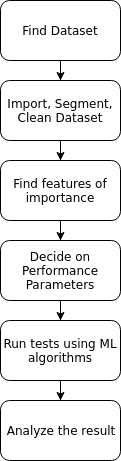
\includegraphics[width=0.2\textwidth]{Chapter3/workflow}\hspace*{\fill}
    \caption{Workflow}
    \label{workflow}
\end{figure}

\section{Dataset}
\paragraph{}
Two popular datasets were found for the purpose of training and testing IDSs, the KDD'99 \cite{kdd99} and the UNSW-NB15 \cite{unsw15}. KDD'99 presented various problems, such as redundancy, unbalanced sets etc., as discussed thoroughly in \cite{unsw_comparison}. UNSW-NB15, besides being a more recent dataset, hence meeting the present standards in types of data packet and more accurate labels, also addressed issues in the KDD'99 dataset. Hence, the choice of UNSW-NB15 was made for this work.

\section{Cleaning the Dataset}
\paragraph{}
The UNSW-NB15 dataset contains over 2.5 million records, and is split into 4 subsets, each containing 700,000 records. The first subset has been used for training the models, and the second for testing throughout the work. Each subset goes through the following steps before it can be used for building the models:
\begin{enumerate}
    \item Import dataset using python Pandas library
    \item Fill empty values (attack\_cat = '' for normal data) with 0
    \item Transform nominal data values to numeric
    \item Add feature names to the Pandas dataframe (only for readability while debugging)
\end{enumerate}

\section{Feature Selection}
\label{feature_select}
\paragraph{}
Decision Tree algorithms in scikit-learn library assign an importance score to each feature on the basis of how much they contribute in the classification. The ExtraTreesClassifier class was used to fetch these importance scores (Figure \ref{feature_importance})
\begin{figure}[h]
    \hfill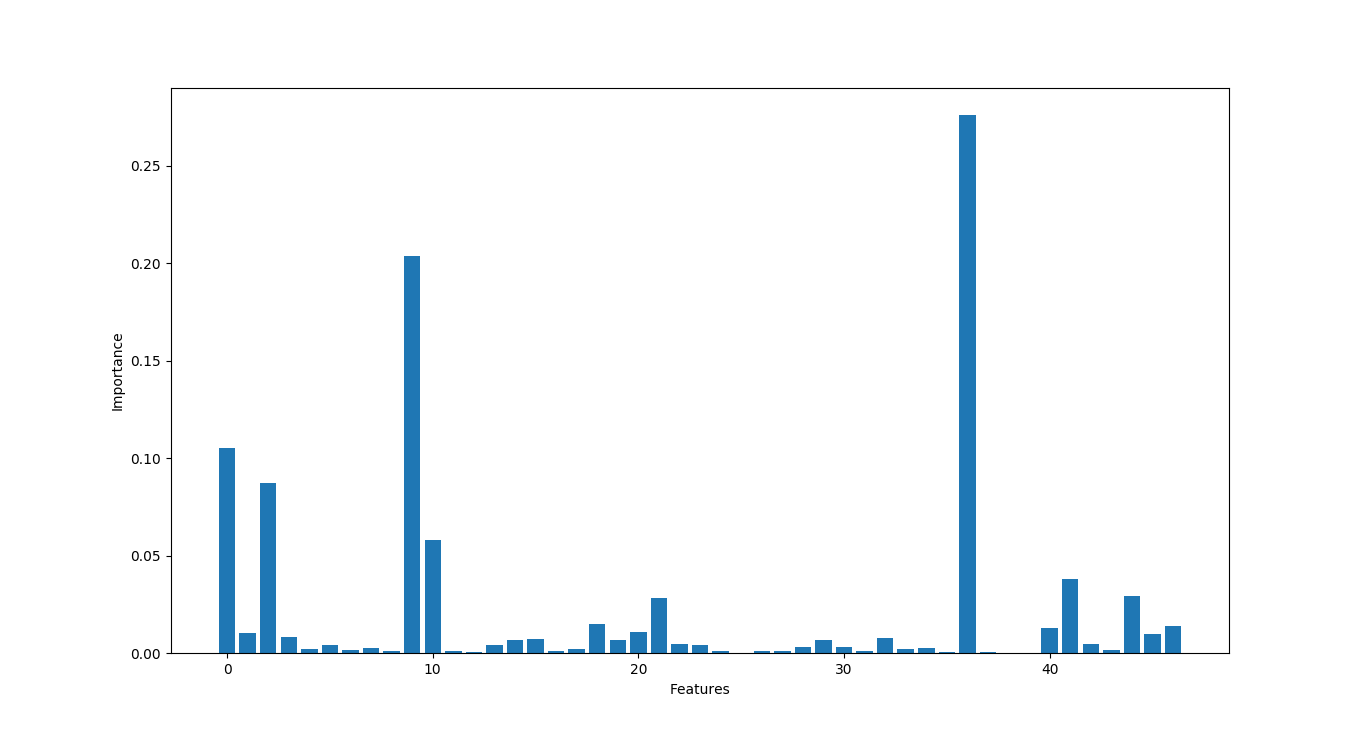
\includegraphics[width=1\textwidth]{Chapter3/feature_importance}\hspace*{\fill}
    \caption{Feature importance}
    \label{feature_importance}
\end{figure}

\paragraph{}
It was observed that 2 features had radically high importance scores (sttl and ct\_state\_ttl). The first one is the source to destination time to live, which is understandable as it is often manipulated to run various kinds of attacks, and the second is an additional generated feature dependent on state, sttl and dttl.

\paragraph{}
The two other peaks in the graph (Figure \ref{feature_importance}), at x = 0 and 2 are source and destination IP addresses. It is understandable that they have a high score as attacks or normal data are likely to originate from the same source and go to the same destination in the dataset curated at a lab at a university. However, it is not very useful to build a generic model to classify an attack as it is a property of the source, and not the kind of data packet.

\section{Performance Parameters}
\paragraph{}
A confusion matrix is used to define accuracy of the models. A confusion matrix has 4 parameters:
\begin{itemize}
    \item True Positive (TP): Number of correctly classified attack records
    \item True Negative (TN): Number of correctly classified normal records
    \item False Positive (FP): Number of misclassified attack records
    \item False Negative (FN): Number of misclassified normal records
\end{itemize}
Using these 4 parameters, the accuracy may be calculated as:
\begin{equation}
    accuracy = \frac {TP + TN} {TP + TN + FP + FN}
\end{equation}

\paragraph{}
To factor in the time of execution, two new parameters are introduced. Since the objective is to maximize accuracy and minimize time of execution, the final score of a model is defined as:
\begin{equation}
    score \propto \frac {accuracy} {execution\_time}
\end{equation}
With the proportionality constant as 1, the Training Score (TS) and Prediction Score (PS) are defined as:
\begin{equation}
    TS = \frac {accuracy} {time\_to\_fit/train}
\end{equation}
\begin{equation}
    PS = \frac {accuracy} {time\_to\_predict/classify}
\end{equation}

\chapter{Results and Observations}
\label{ch:SC}

\paragraph{}
The KNN Classifier was tested with the value of k = 1 to reduce the number of computations as much as possible to speed up the process. All decision tree based classifiers have been tested with max\_depth = 2 and 4. This parameter defines how deep the tree can build itself. In the case of DecisionTreeClassifier, max\_depth = None has also been considered. The execution time and accuracy for each model is presented in Table \ref{res_all} and Table \ref{res_2}

\begin{table}[h]
    \caption{Execution times of different models with all features}
    \centering
    \label{res_all}
    \begin{tabular}{| l | r | r | r |}
        \hline
        \textbf{Model} & \textbf{TTF (sec)} & \textbf{TTP (sec)} & \textbf{Accuracy} \\
        \hline
        KNeighborsClassifier(n\_neighbors = 1) & 78.721 & 54.251 & 0.9519 \\
        \hline
        GaussianNB() & 0.752 & 0.77 & 0.9181 \\
        \hline
        DecisionTreeClassifier() & 3.76 & 0.3 & 0.9746 \\
        \hline
        DecisionTreeClassifier(max\_depth = 2) & 3.463 & 0.295 & 0.9873 \\
        \hline
        DecisionTreeClassifier(max\_depth = 4) & 3.781 & 0.32 & 0.9876 \\
        \hline
        RandomForestClassifier(max\_depth = 2) & 4.666 & 0.472 & 0.9885 \\
        \hline
        RandomForestClassifier(max\_depth = 4) & 7.144 & 0.521 & 0.99 \\
        \hline
        ExtraTreesClassifier(max\_depth = 2) & 1.167 & 0.489 & 0.9276 \\
        \hline
        ExtraTreesClassifier(max\_depth = 4) & 1.604 & 0.551 & 0.9617 \\
        \hline
    \end{tabular}
\end{table}

\begin{table}[h]
    \caption{Execution times of different models with 2 selected features}
    \centering
    \label{res_2}
    \begin{tabular}{| l | r | r | r |}
        \hline
        \textbf{Model} & \textbf{TTF (sec)} & \textbf{TTP (sec)} & \textbf{Accuracy} \\
        \hline
        KNeighborsClassifier(n\_neighbors = 1) & 0.909 & 0.192 & 0.9895 \\
        \hline
        GaussianNB() & 0.073 & 0.039 & 0.9860 \\
        \hline
        DecisionTreeClassifier() & 0.057 & 0.013 & 0.9895 \\
        \hline
        DecisionTreeClassifier(max\_depth = 2) & 0.075 & 0.023 & 0.98733 \\
        \hline
        DecisionTreeClassifier(max\_depth = 4) & 0.195 & 0.013 & 0.9895 \\
        \hline
        RandomForestClassifier(max\_depth = 2) & 0.902 & 0.192 & 0.9885 \\
        \hline
        RandomForestClassifier(max\_depth = 4) & 1.027 & 0.219 & 0.9895 \\
        \hline
        ExtraTreesClassifier(max\_depth = 2) & 0.55 & 0.198 & 0.9826 \\
        \hline
        ExtraTreesClassifier(max\_depth = 4) & 0.654 & 0.221 & 0.9895 \\
        \hline
    \end{tabular}
\end{table}

\paragraph{}
To understand the difference in the performance of these models, a better visualization of the data in Table \ref{res_all} and Table \ref{res_2} is presented in Figure \ref{ttf_improvement}, Figure \ref{ttp_improvement} and Figure \ref{acc_improvement}.

\begin{figure}[h]
    \hfill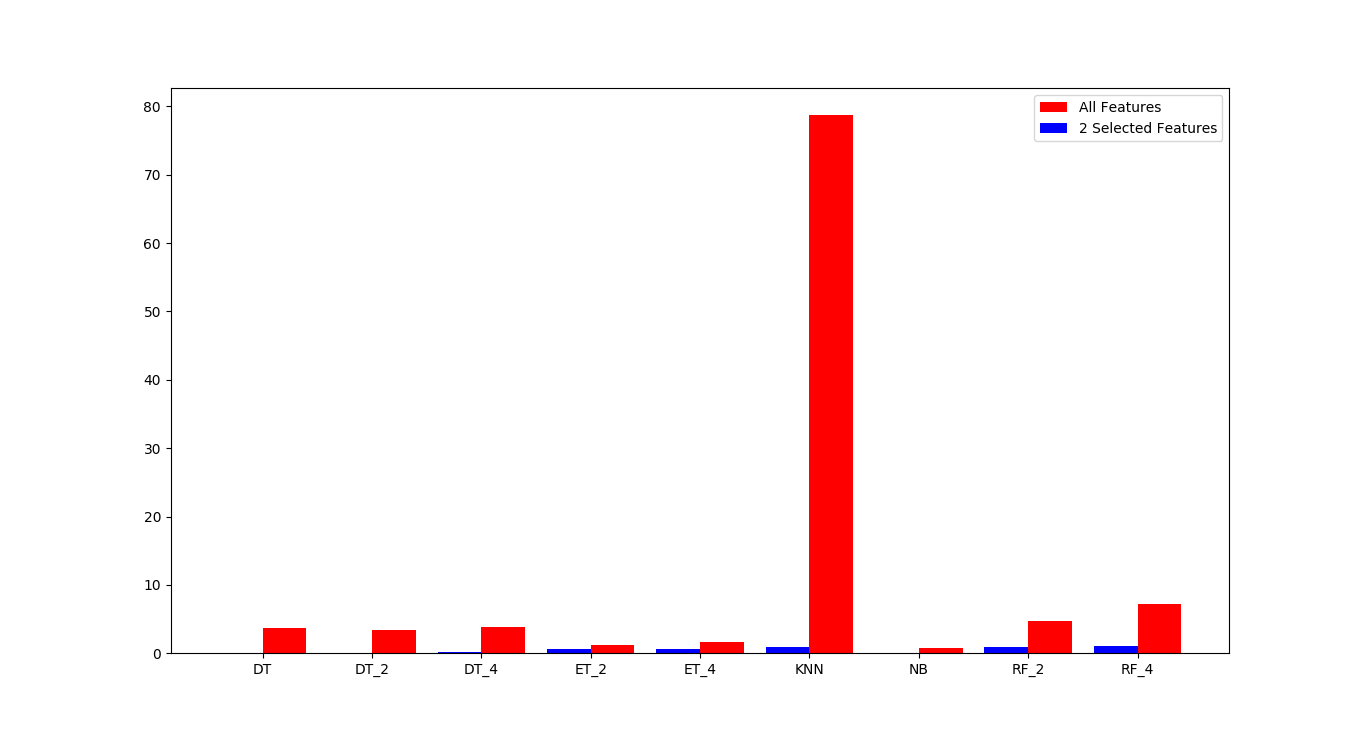
\includegraphics[width=1\textwidth]{Chapter4/ttf_improvement}\hspace*{\fill}
    \caption{Change in TTF of different models (lower is better)}
    \label{ttf_improvement}
\end{figure}

\begin{figure}[h]
    \hfill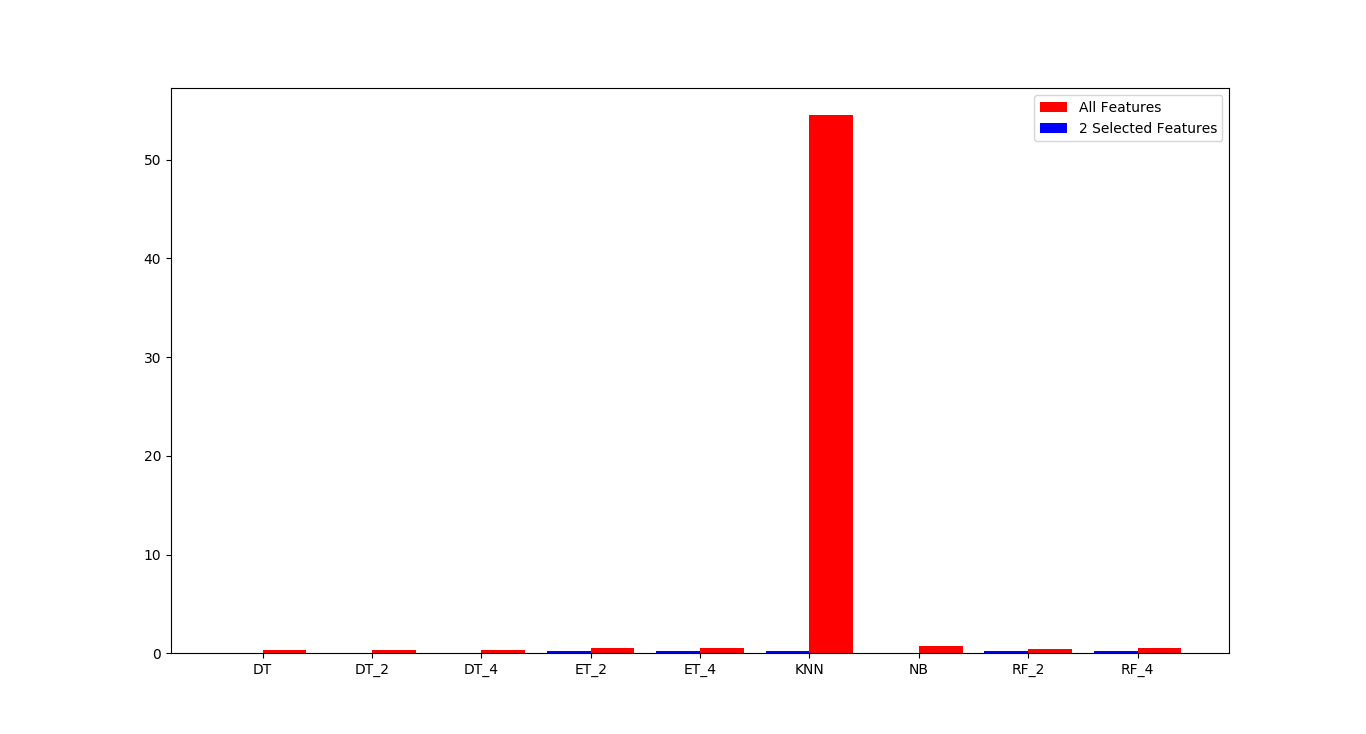
\includegraphics[width=1\textwidth]{Chapter4/ttp_improvement}\hspace*{\fill}
    \caption{Change in TTP of different models (lower is better)}
    \label{ttp_improvement}
\end{figure}

\begin{figure}[h]
    \hfill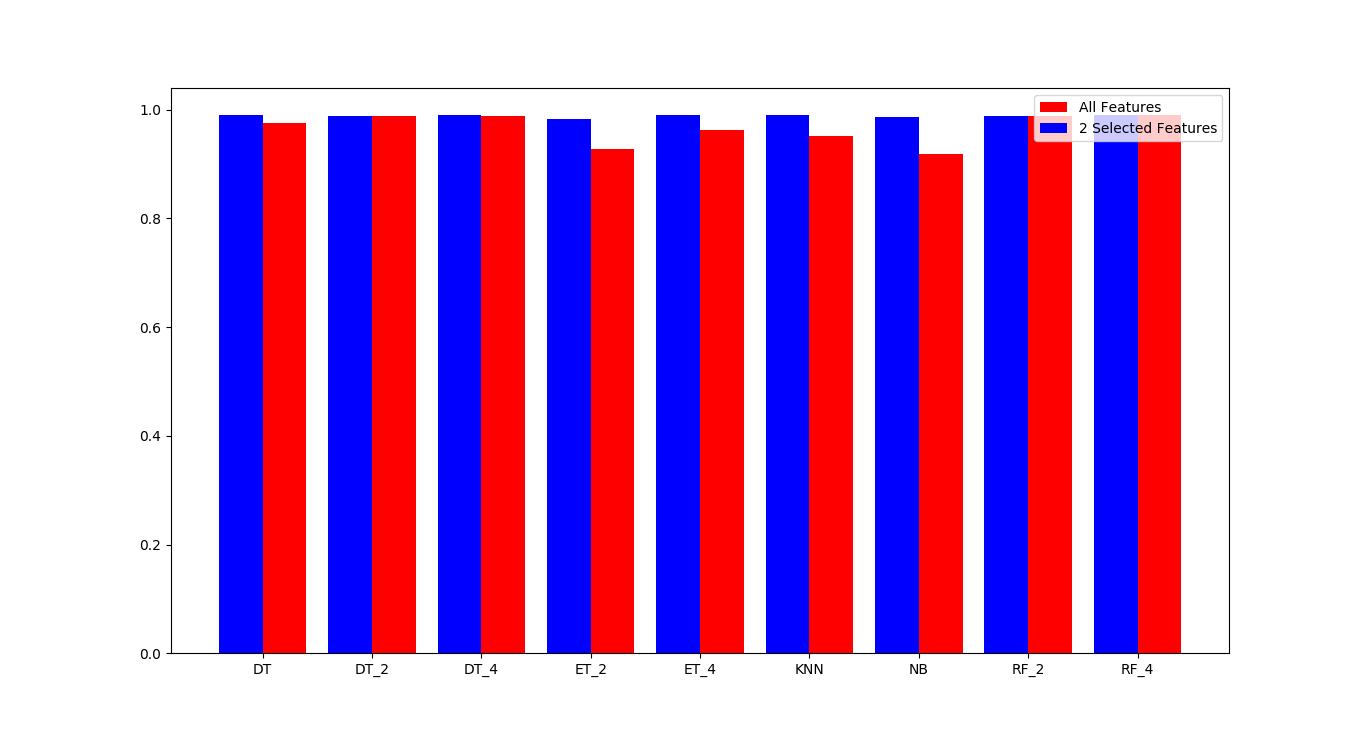
\includegraphics[width=1\textwidth]{Chapter4/acc_improvement}\hspace*{\fill}
    \caption{Change in Accuracy of different models (higher is better)}
    \label{acc_improvement}
\end{figure}

\paragraph{}
It is clear from these results that selecting the 2 features mentioned in Section \ref{feature_select} resulted in radically reduced execution times, especially for KNN (77.812 seconds reduced), without negatively affecting to the accuracy of the models. Most models see only slight change in accuracy, but the change itself is usually positive. The reduction in execution time resulted in significant improvement in the Training and Prediction Scores (Table \ref{final_scores}).

\begin{table}
    \caption{Training and Prediction Scores}
    \label{final_scores}
    \begin{tabular}{| l | r | r | r | r |}
        \hline
         & \multicolumn{2}{c |}{\textbf{All Features}} & \multicolumn{2}{c |}{\textbf{2 Features}} \\
        \hline
        \textbf{Model} & \textbf{TS} & \textbf{PS} & \textbf{TS} & \textbf{PS} \\
        \hline
        KNeighborsClassifier(n\_neighbors = 1) & 0.012 & 0.017 & 1.088 & 5.153 \\
        \hline
        GaussianNB() & 1.22 & 1.192 & 13.507 & 25.282 \\
        \hline
        DecisionTreeClassifier() & 0.259 & 3.248 & 17.359 & 76.115 \\
        \hline
        DecisionTreeClassifier(max\_depth = 2) & 0.285 & 3.346 & 13.164 & 42.927 \\
        \hline
        DecisionTreeClassifier(max\_depth = 4) & 0.261 & 3.086 & 5.074 & 76.115 \\
        \hline
        RandomForestClassifier(max\_depth = 2) & 0.211 & 2.094 & 1.095 & 5.148 \\
        \hline
        RandomForestClassifier(max\_depth = 4) & 0.138 & 1.9 & 0.963 & 4.518 \\
        \hline
        ExtraTreesClassifier(max\_depth = 2) & 0.794 & 1.896 & 1.786 & 4.962 \\
        \hline
        ExtraTreesClassifier(max\_depth = 4) & 0.599 & 1.745 & 1.513 & 4.477 \\
        \hline
    \end{tabular}
\end{table}

\begin{table}
    \caption{Confusion Matrix for the models}
    \centering
    \label{confusion_matrix}
    \begin{tabular}{| l | r | r | r | r |}
        \hline
        \textbf{Model} & \textbf{TN} & \textbf{FN} & \textbf{FP} & \textbf{TP} \\
        \hline
        KNN & 639191 & 25586 & 8060 & 27163 \\
        \hline
        KNN & 640364 & 463 & 6887 & 52286 \\
        \hline
        NB & 641671 & 51709 & 5580 & 1040 \\
        \hline
        NB & 637461 & 0 & 9790 & 52749 \\
        \hline
        DT & 642239 & 12715 & 5012 & 40034 \\
        \hline
        DT & 640364 & 462 & 6887 & 52287 \\
        \hline
        DT\_2 & 638630 & 248 & 8621 & 52501 \\
        \hline
        DT\_2 & 638630 & 248 & 8621 & 52501 \\
        \hline
        DT\_4 & 638740 & 146 & 8511 & 52603 \\
        \hline
        DT\_4 & 640364 & 463 & 6887 & 52286 \\
        \hline
        RF\_2 & 639520 & 278 & 7731 & 52471 \\
        \hline
        RF\_2 & 639537 & 284 & 7714 & 52465 \\
        \hline
        RF\_4 & 642116 & 1837 & 5135 & 50912 \\
        \hline
        RF\_4 & 640364 & 463 & 6887 & 52286 \\
        \hline
        ET\_2 & 645241 & 48667 & 2010 & 4082 \\
        \hline
        ET\_2 & 639942 & 4829 & 7309 & 47920 \\
        \hline
        ET\_4 & 644140 & 23672 & 3111 & 29077 \\
        \hline
        ET\_4 & 640371 & 468 & 6880 & 52281 \\
        \hline
    \end{tabular}
\end{table}

\paragraph{}
The data in Table \ref{final_scores} is presented in Figure \ref{ps_improvement} and Figure \ref{ts_improvement} for visualizing the change in the Training and Prediction Scores. It is evident from these results that the two selected features in the dataset are indeed contributing the most in the classification. Accuracy and execution time improved upon ignoring the other features. The time reduction is because there are less dimensions in the feature space for the models to process, while the accuracy improvement may suggest that the other features had a slight negative contribution in the classification. A closer look at the confusion matrix results (Table \ref{confusion_matrix}) suggests that, although the overall accuracy has improved, the false positive rate in most cases has increased.

\begin{figure}[h]
    \hfill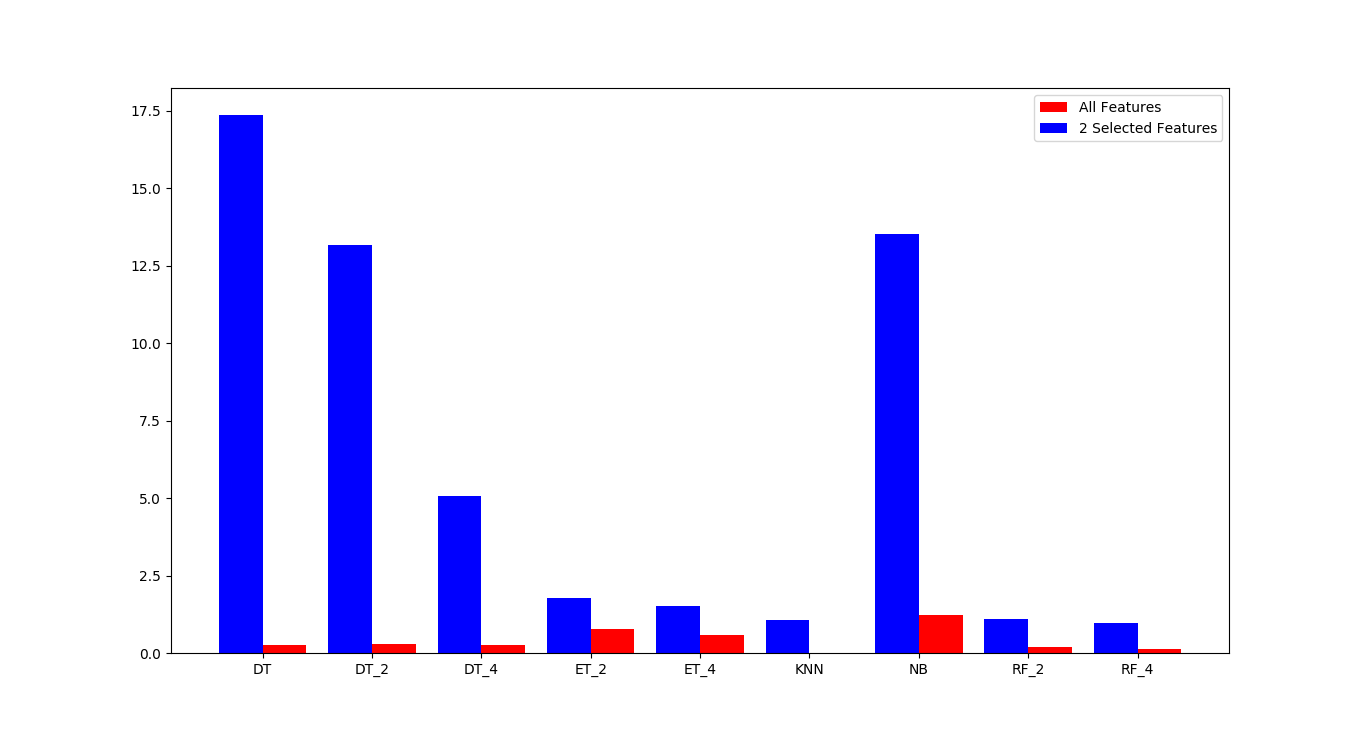
\includegraphics[width=1\textwidth]{Chapter4/ts_improvement}\hspace*{\fill}
    \caption{Change in TS of different models (higher is better)}
    \label{ts_improvement}
\end{figure}

\begin{figure}[h]
    \hfill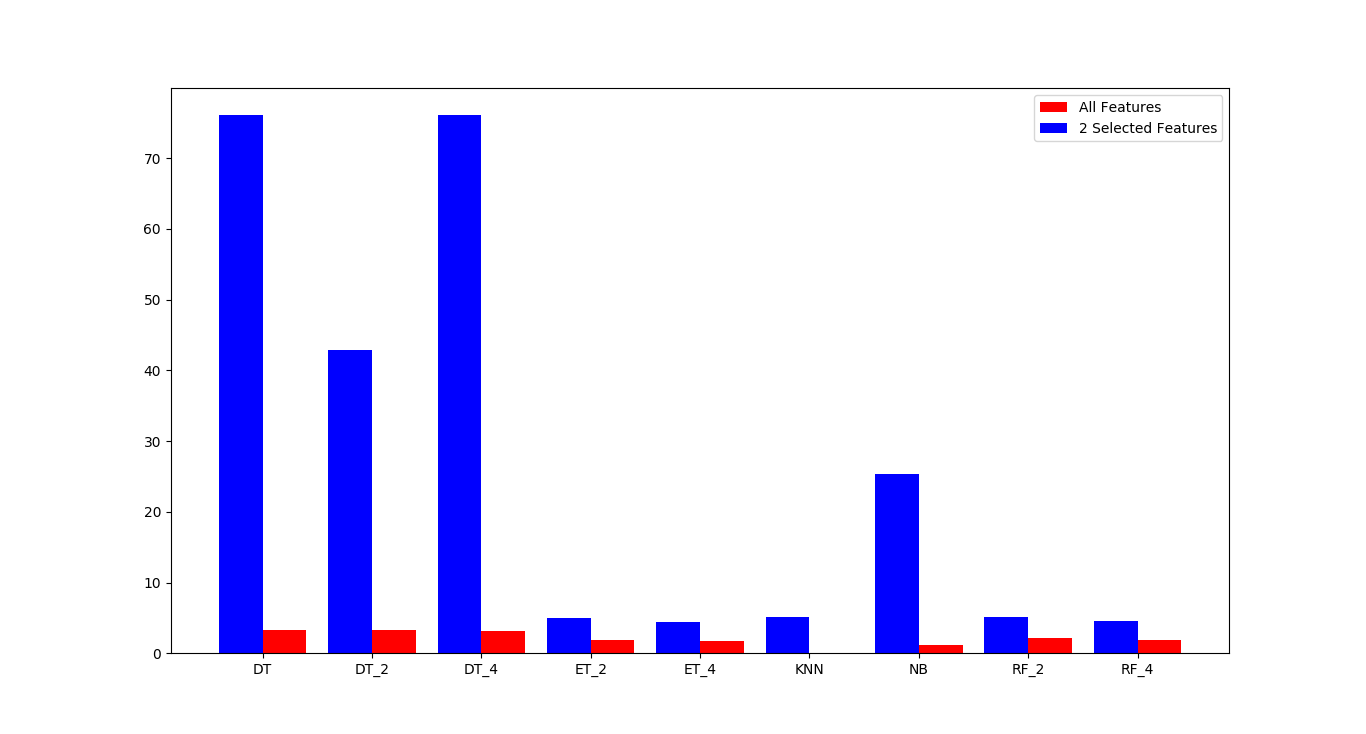
\includegraphics[width=1\textwidth]{Chapter4/ps_improvement}\hspace*{\fill}
    \caption{Change in PS of different models (higher is better)}
    \label{ps_improvement}
\end{figure}

\chapter{Result Analysis and Conclusion}

\section{Result Analysis}

\subsection{Useful features in Intrusion Detection}

\paragraph{}
It is evident from this study that the basic features, such as source to destination time to live, destination to source time to live and state of the data packet are few of the most important features for intrusion detection. However, relying on them completely may lead to a system which may not respond to growing trends in cyber-security. This, however, can be because most of the attacks classified in UNSW-NB15 dataset use exploits related to these basic features. If other features are completely ignored and attackers figure out ways to exploit those features, it will become impossible to detect those intrusions in the future. It is important to update the list of important features by running periodic tests over fresh data.

\subsection{Notes about the different models}

\paragraph{}
A few interesting cases came up durnig the tests.
\begin{itemize}
    \item The GaussianNB classifier, when tested with all features, had the lowest execution time, and the lowest accuracy. This is because GaussianNB works under the assumption that the features are not related to each other. There is minimal computation resulting in lower time signatures and since the assumption is not realistic, the accuracy lowered. When tested with the 2 selected features, however, while the execution time remained comparable to other models, the accuracy increased significantly. This increase in accuracy can be attributed to the low dimensionality of the dataset with just 2 features making the assumption more realistic than before.
    \item Decision Tree classifier with max-depth 2, gave the exact same predictions when tested with all features and when tested with only 2 features. This is because the optimization done with the feature selection is used automatically by the Decision Tree algorithm. The extra time used with all features must be due to the process of selecting these features. Since there are only 2 features which are selected, max-depth of 2 gives an optimal classification result. (Figure \ref{dtc_md2_2_features})
\end{itemize}

\begin{figure}[h]
    \hfill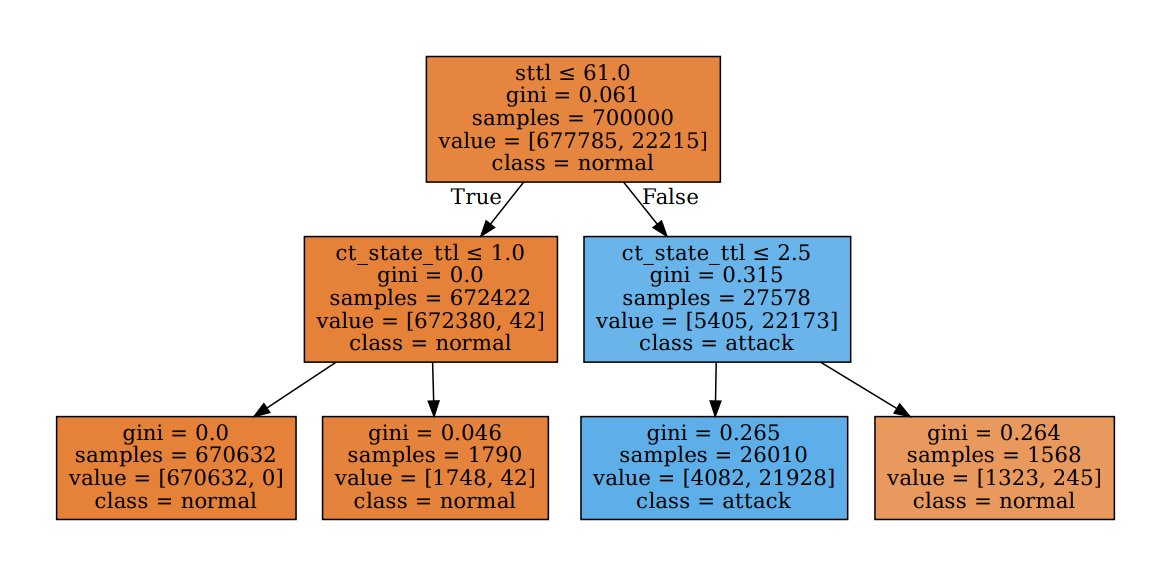
\includegraphics[width=1\textwidth]{Chapter5/dtc_md2_2_features}\hspace*{\fill}
    \caption{Decision Tree with max-depth = 2 tested with 2 features}
    \label{dtc_md2_2_features}
\end{figure}

\section{Conclusion}

\paragraph{}
Given that the UNSW-NB15 is a realistic dataset, the results from these models suggest Decision Trees as the most optimal model to implement an IDS in a low powered environment. The optimization done using feature selection, however, is not very reliable. The results suggest that most cyber attacks exploit similar features (sttl, dttl, state etc. as mentioned in Section \ref{unsw_details}). Since the results were obtained through analysis over a static dataset, the importance of the two selected features will require further testing on live data.

\subsection{Future Scope}

\paragraph{}
 More tests must be conducted to find an optimal value for the internal parameters of Decision Trees, such as max-depth. The radical improvement in performance from the two selected features is very convincing, however choosing the right features will be dependent on the type of data going in as input into the system and the way they are distributed. The correct features may vary from network to network, and extreme care must be taken while implementing such a model.

\paragraph{}
Tests must be conducted on live data and small devices, which are the focus of this work. The results from this work may act as a starting point to further research in this domain.

\chapter{Chapter Title}

\section{vvvvv}
\chapter{Conclusion}
\section{fff}

\addappheadtotoc
\appendixpage
\begin{appendix}

\chapter{Code (if required)}
\section{Kerberos Protocol}
\scriptsize{
\begin{verbatim}
MODULE main

VAR

--Creating agents which are to type agtype
agA : agtype; 
agB : agtype;
agS : agtype;
agI : agtype;
Iactive: boolean;

--Assigning initial to values to all variables

ASSIGN
init(agA.state):=wait;
init(agB.state):=wait;
init(agS.state):=wait;
init(agI.state):=wait;
init(agA.count):=0;
init(agB.count):=0;
init(agS.count):=0;
init(agI.count):=0;
init(agA.authenticated):=FALSE;
init(agB.authenticated):=FALSE;
init(agI.authenticated):=FALSE;
init(agS.authenticated):=TRUE;

--Transitions for the variable indicating presence or absence of intruder

next(Iactive):=
case
!Iactive:{0,1};
Iactive & agI.state=receive4beta:{0,1};
1:Iactive;
esac;

--Transitions for agent A's state

next(agA.state):=
case
agA.state=wait: send1;
agS.state=send2 & agA.state=send1: receive2;
agA.state=receive2: send3alpha;
agB.state=send4alpha & agA.state=send3alpha: receive4alpha;
agA.state=receive4alpha: wait;
1:agA.state;
esac;

--Transitions for agent B's state

next(agB.state):=
case
agA.state=send3alpha & agB.state=wait: receive3alpha;
agI.state=send3beta & agB.state=wait & Iactive: receive3beta;
agI.state=send3beta & agB.state=send4alpha & Iactive: receive3beta;
agB.state=receive3alpha:send4alpha;
agB.state=receive3beta:send4beta;
agB.state=send4alpha:wait;
1:agB.state;
esac;

--Transitions for Server S's state

next(agS.state):=
case
agA.state=send1 & agS.state=wait: receive1;
agS.state=receive1:send2;
agS.state=send2:wait;
1:agS.state;
esac;

--Transitions for the Intruder's state

next(agI.state):=
case
agI.state=wait & agA.state=send3alpha & agB.state=wait & Iactive: receive3beta;
agI.state=receive3beta & Iactive: send3beta;
agI.state=send3beta & agB.state=send4beta & Iactive  : receive4beta;
agI.state=receive4beta & Iactive: wait;
1:agI.state;
esac;

--Transitions for Agent A's counter

next(agA.count):=
case
agA.state=send1|agA.state=receive2: agA.count;
agA.state=send3alpha & agA.count<1:agA.count+1;
agA.count=1 & agA.state=receive2: 0;
1:agA.count;
esac;

--Transitions for Agent B's counter

next(agB.count):=
case
agB.state=receive3beta & agB.count<2|agB.state=receive3alpha & agB.count<2: agB.count+1;
agB.state=send4alpha |agB.state=send4beta:agB.count;
agB.count=1 & agA.state=receive4alpha & !Iactive:0;
agB.count=2 & agA.state=send3alpha|agB.count=1 & agA.state=send3alpha: 0;
1:agB.count;
esac;

--Transitions for Agent I's counter

next(agI.count):=
case
agI.state=receive3beta & agI.count<2 & Iactive:agI.count+1;
agI.state=send3beta & Iactive:agI.count;
agI.state=receive4beta & agI.count<2 & Iactive: agI.count+1;
agI.count=2: 0;
1:agI.count;
esac;

--Transitions for variable indicating agent A's authentication

next(agA.authenticated):=
case
agA.state=receive4alpha :TRUE;
1:agA.authenticated;
esac;

--Transitions for variable indicating agent B's authentication

next(agB.authenticated):=
case
agB.state=send4alpha |agB.state=send4beta :TRUE;
1:agB.authenticated;
esac;

--Transitions for variable indicating agent B's authentication which 
--indicates that it has received the fourth message

next(agI.authenticated):=
case
agI.state=receive4beta :TRUE;
1:agI.authenticated;
esac;

--Agent S always is authenticated so transitions to the false state do not occur

next(agS.authenticated):=
case
1:agS.authenticated;
esac;

--Specifications which detect the presence of replay attack

--Agent B should not receive more messages than what agent A has sent it
--SPEC AG!(agA.count < agB.count);

--Agent I should never receive the fourth message
SPEC AG!(agI.state=receive4beta);

--Module for each agent's type which includes the agent's state variable, 
--its counter and its authentication variable

MODULE agtype

VAR
state: {wait, send1, receive1, send2,receive2, 
send3alpha, send3beta, receive3alpha, receive3beta, 
send4alpha,send4beta, receive4alpha, receive4beta };
count:{0,1,2};
authenticated:boolean;

\end{verbatim}


\section{Kerberos Protocol with Freshness Concept}
\begin{verbatim}
MODULE main

VAR

--Creating agents which are to type agtype
agA : agtype; 
agB : agtype;
agS : agtype;
agI : agtype;
Iactive: boolean;
Fresh:0..20;
Time:0..20;

--Assigning initial to values to all variables
 
ASSIGN
init(agA.state):=wait;
init(agB.state):=wait;
init(agS.state):=wait;
init(agI.state):=wait;
init(agA.count):=0;
init(agB.count):=0;
init(agS.count):=0;
init(agI.count):=0;
init(agA.authenticated):=FALSE;
init(agB.authenticated):=FALSE;
init(agI.authenticated):=FALSE;
init(agS.authenticated):=TRUE;
init(Fresh):=0;
init(Time):=0;

--Transitions for the variable indicating presence or absence of intruder

next(Iactive):=
case
!Iactive:{0,1};
Iactive & agI.state=receive4beta:{0,1};
1:Iactive;
esac;

--Transitions for agent A's state

next(agA.state):=
case
agA.state=wait: send1;
agS.state=send2 & agA.state=send1: receive2;
agA.state=receive2: send3alpha;
agB.state=send4alpha & agA.state=send3alpha: receive4alpha;
agA.state=receive4alpha: wait;
1:agA.state;
esac;

--Transitions for agent B's state

next(agB.state):=
case
agA.state=send3alpha & agB.state=wait & Fresh=0: receive3alpha;
agI.state=send3beta & agB.state=wait & Iactive & Fresh=0: receive3beta;
agI.state=send3beta & agB.state=send4alpha & Iactive & Fresh=0: receive3beta;
agB.state=receive3alpha:send4alpha;
agB.state=receive3beta:send4beta;
agB.state=send4alpha:wait;
1:agB.state;
esac;

--Transitions for Server S's state

next(agS.state):=
case
agA.state=send1 & agS.state=wait: receive1;
agS.state=receive1:send2;
agS.state=send2:wait;
1:agS.state;
esac;

--Transitions for the Intruder's state

next(agI.state):=
case
agI.state=wait & agA.state=send3alpha & agB.state=wait & Iactive: receive3beta;
agI.state=receive3beta & Iactive: send3beta;
agI.state=send3beta & agB.state=send4beta & Iactive  : receive4beta;
agI.state=receive4beta & Iactive: wait;
agI.state=send3beta & Time>2: wait;
1:agI.state;
esac;

--Transitions for Agent A's counter

next(agA.count):=
case
agA.state=send1|agA.state=receive2: agA.count;
agA.state=send3alpha & agA.count<1:agA.count+1;
agA.count=1 & agA.state=receive2: 0;
1:agA.count;
esac;

--Transitions for Agent B's counter

next(agB.count):=
case
agB.state=receive3beta & agB.count<2|agB.state=receive3alpha & agB.count<2: agB.count+1;
agB.state=send4alpha|agB.state=send4beta:agB.count;
agB.count=1 & agA.state=receive4alpha & !Iactive:0;
agB.count=2 & agA.state=send3alpha|agB.count=1 & agA.state=send3alpha: 0;
1:agB.count;
esac;

--Transitions for Agent I's counter

next(agI.count):=
case
agI.state=receive3beta & agI.count<2 & Iactive:agI.count+1;
agI.state=send3beta & Iactive:agI.count;
agI.state=receive4beta & agI.count<2 & Iactive: agI.count+1;
agI.count=2: 0;
1:agI.count;
esac;

--Transitions for variable indicating agent A's authentication

next(agA.authenticated):=
case
agA.state=receive4alpha :TRUE;
1:agA.authenticated;
esac;

--Transitions for variable indicating agent B's authentication

next(agB.authenticated):=
case
agB.state=send4alpha|agB.state=send4beta :TRUE;
1:agB.authenticated;
esac;

--Transitions for variable indicating agent B's authentication which 
--indicates that it has received the fourth message

next(agI.authenticated):=
case
agI.state=receive4beta :TRUE;
1:agI.authenticated;
esac;

--Agent S always is authenticated so transitions to the false state do not occur

next(agS.authenticated):=
case
1:agS.authenticated;
esac;

--Transitions for the freshness variable

next(Fresh):=
case
agA.state=send3alpha & agB.state=wait:0;
Fresh<20:Fresh+1;
1:0;
esac;

--Transitions for the Intruder's timer variable

next(Time):=
case
agI.state=receive3beta:0;
Time<20:Time+1;
1:0;
esac;

--Specifications which detect the presence of replay attack

--Agent B should not receive more messages than what agent A has sent it
SPEC AG!(agA.count < agB.count);

--Agent I should never receive the fourth message
SPEC AG!(agI.state=receive4beta);

--Module for each agent's type which includes the agent's state variable, 
--its counter and its authentication variable

MODULE agtype

VAR
state:{wait, send1, receive1, send2,receive2, 
send3alpha, send3beta, receive3alpha, receive3beta, 
send4alpha, send4beta, receive4alpha, receive4beta};
count:{0,1,2};
authenticated:boolean;

\end{verbatim}

\chapter{Trace Files}

\section{Replay Attack}
\begin{verbatim}
-- specification AG !(agA.count < agB.count)  is false
-- as demonstrated by the following execution sequence
Trace Description: CTL Counterexample 
Trace Type: Counterexample 
-> State: 1.1 <-
  agA.state = wait
  agA.count = 0
  agA.authenticated = 0
  agB.state = wait
  agB.count = 0
  agB.authenticated = 0
  agS.state = wait
  agS.count = 0
  agS.authenticated = 1
  agI.state = wait
  agI.count = 0
  agI.authenticated = 0
  Iactive = 0
-> Input: 1.2 <-
-> State: 1.2 <-
  agA.state = send1
  agS.count = 2
-> Input: 1.3 <-
-> State: 1.3 <-
  agS.state = receive1
-> Input: 1.4 <-
-> State: 1.4 <-
  agS.state = send2
-> Input: 1.5 <-
-> State: 1.5 <-
  agA.state = receive2
  agS.state = wait
-> Input: 1.6 <-
-> State: 1.6 <-
  agA.state = send3alpha
  Iactive = 1
-> Input: 1.7 <-
-> State: 1.7 <-
  agA.count = 1
  agB.state = receive3alpha
  agI.state = receive3beta
-> Input: 1.8 <-
-> State: 1.8 <-
  agB.state = send4alpha
  agB.count = 1
  agI.state = send3beta
  agI.count = 1
-> Input: 1.9 <-
-> State: 1.9 <-
  agA.state = receive4alpha
  agB.state = receive3beta
  agB.authenticated = 1
-> Input: 1.10 <-
-> State: 1.10 <-
  agA.state = wait
  agA.authenticated = 1
  agB.state = send4beta
  agB.count = 2
-- specification AG !(agI.state = receive4beta)  is false
-- as demonstrated by the following execution sequence
Trace Description: CTL Counterexample 
Trace Type: Counterexample 
-> State: 2.1 <-
  agA.state = wait
  agA.count = 0
  agA.authenticated = 0
  agB.state = wait
  agB.count = 0
  agB.authenticated = 0
  agS.state = wait
  agS.count = 0
  agS.authenticated = 1
  agI.state = wait
  agI.count = 0
  agI.authenticated = 0
  Iactive = 0
-> Input: 2.2 <-
-> State: 2.2 <-
  agA.state = send1
  agS.count = 2
-> Input: 2.3 <-
-> State: 2.3 <-
  agS.state = receive1
-> Input: 2.4 <-
-> State: 2.4 <-
  agS.state = send2
-> Input: 2.5 <-
-> State: 2.5 <-
  agA.state = receive2
  agS.state = wait
-> Input: 2.6 <-
-> State: 2.6 <-
  agA.state = send3alpha
  Iactive = 1
-> Input: 2.7 <-
-> State: 2.7 <-
  agA.count = 1
  agB.state = receive3alpha
  agI.state = receive3beta
-> Input: 2.8 <-
-> State: 2.8 <-
  agB.state = send4alpha
  agB.count = 1
  agI.state = send3beta
  agI.count = 1
-> Input: 2.9 <-
-> State: 2.9 <-
  agA.state = receive4alpha
  agB.state = receive3beta
  agB.authenticated = 1
-> Input: 2.10 <-
-> State: 2.10 <-
  agA.state = wait
  agA.authenticated = 1
  agB.state = send4beta
  agB.count = 2
-> Input: 2.11 <-
-> State: 2.11 <-
  agA.state = send1
  agI.state = receive4beta

\end{verbatim}

\section{Replay Attack overcome using Freshness Concept}

\begin{verbatim}
-- specification AG !(agA.count < agB.count)  is true
-- specification AG !(agI.state = receive4beta)  is true

\end{verbatim}

}
\end{appendix}



\addcontentsline{toc}{chapter}{References}
\renewcommand{\bibname}{References} % changes default name Bibliography to References
\bibliographystyle{IEEEtran} % bibliography style
\bibliography{References/myref} % References file

\rhead{}
\addcontentsline{toc}{chapter}{ProjectDetail}

%=========Enter the required details=================================================
\begin{table}
\begin{scriptsize}
\caption{Project Detail}
\begin{tabularx}{\textwidth}{|X|X|X|X|}
\multicolumn{4}{l}{\textit{Student Details}}\\
\hline
\textbf{Student Name}&\multicolumn{2}{X}{Pratyay Amrit}&\\ \hline
Registration Number&140953430&Section/Roll No.& B/61\\ \hline
Email Address&\tiny{p.amrit@live.com}&Phone No.(M)&7795443730 \\  \hline
% \textbf{Student Name}&\multicolumn{2}{X}{Your Name}&\\ \hline
% Registration Number&070911001&Section/Roll No.& A/01\\ \hline
% Email Address&\tiny{yourname@yahoo.com}&Phone No.(M)&9891000000 \\  \hline
%\textbf{Student Name}&\multicolumn{2}{X}{Your Name}&\\ \hline
%Registration Number&070911001&Section/Roll No.& A/01\\ \hline
%Email Address&\tiny{yourname@yahoo.com}&Phone No.(M)&9891000000 \\  \hline
\multicolumn{4}{l}{\textit{Project Details}}\\ \hline
\textbf{Project Title}&\multicolumn{2}{c}{\tiny{Intrusion Detection Systems for Use in Low-Powered Devices}}& \\ \hline
Project Duration& 4 Months&Date of Reporting& 08-05-2018 \\ \hline
% \multicolumn{4}{l}{\textit{Organization Details}}\\ \hline
% \textbf{Organization Name}&\multicolumn{2}{c}{Name of your organization}& \\ \hline
% Full Postal Address&\multicolumn{2}{X}{Whitefield, B'lore} &\\ \hline
% Website Address&\multicolumn{2}{X}{www.abc.com} &\\ \hline
% \multicolumn{4}{l}{\textit{Supervisor Details}}\\ \hline
% \textbf{Supervisor Full Name}&\multicolumn{2}{X}{Name}& \\ \hline
% Designation&\multicolumn{2}{c}{Project Leader or Manager} &\\ \hline
% Full Contact Address with PIN Code&\multicolumn{2}{X}{\#1,Whitefield, B'lore}& \\ \hline
% Email Address&xyz@abc.in&Phone No.(M)&9767541234\\ \hline
\multicolumn{4}{l}{\textit{Internal Guide Details}}\\ \hline
\textbf{Faculty Name}&\multicolumn{2}{X}{Ms. Ipsita Upasana} &\\ \hline
Full Contact Address with PIN Code&\multicolumn{2}{p{6cm}}{Department of Information and Communication Technology,  Manipal Institute of Technology, Manipal-576104}& \\ \hline
Email Address&\multicolumn{2}{c}{ipsita.upasana@manipal.edu}&\\  \hline
\end{tabularx}
\end{scriptsize}
\end{table}


\end{document}
